\chapter{Scheduler}

The Scheduler is one of the widely used list scheduling techniques for commencing operations under hardware constraints. It takes input from the Matlab script after the permutation of the matrix. The operation of the scheduler tool is divided into the following major phases:
\begin{enumerate}
	\item Matrix Data and Hardware Constraints
	\item Symbolic analysis
	\item Scheduling 
\end{enumerate}

\section{Matrix Data and Hardware Constraints}
The Scheduler tool accepts the input matrix data in  Compressed Column Sparse (CCS) format, i.e., generated from MATLAB Scripts. The following hardware constraints are taken into account, which is as follows:
\begin{enumerate}
        \item Number of Data BRAM blocks
        \item Number of MAC(Fused Multiplier) units
        \item Number of DIV(Division) units
        \item Latency of all the units
        \item Number of Data BRAM Ports
        \item Address depth of Data \& Instruction BRAMs
\end{enumerate}
The preprocessing process ensures that the on-chip memory is sufficient to operate.

\section{Symbolic analysis}



The State-of-the-art Gilbert's Transform requires the locations of non-zero elements. Therefore, this includes the need for symbolic analysis. 

The algorithm can be easily understandable by considering the analysis step using the following example:-\\\\
Consider the following matrix with the non-zero Locations red in color whereas zeros' as white color.\\
\begin{figure}[H]
    \centering
    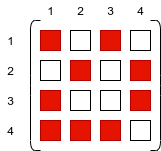
\includegraphics[width = 0.30\textwidth]{./Scheduler/PpT-Symbolic_1.png}
    \caption{A matrix non-zero location}
    \label{fig:Symbolic_1}
\end{figure}

As per Gilbert's algorithm, We will be analyzing column by column. The new fill-in Matrix will be indicated using yellow color.Symbolic Analysis is analyzing data and creating the directed acyclic graph for the floating-point operations.We will be considering \ref{Symbolic_0}

\begin{figure}[H]
    \centering
    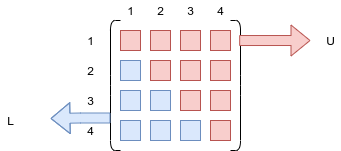
\includegraphics[width = 0.40\textwidth]{./Scheduler/PpT-Symbolic_0.png}
    \caption{Convention of LU Matrix Position}
    \label{fig:Symbolic_0}
\end{figure}



\textbf{Column 1: -}

It is the only column that is guaranteed to have no other additional non-zero elements.
\begin{minipage}{0.45\textwidth}
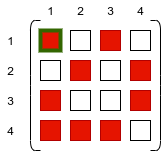
\includegraphics[width=0.45\textwidth]{./Scheduler/PpT-Symbolic_A00.png}
\end{minipage}%
\hfill
\begin{minipage}{0.85\textwidth}
According to equation \ref{eqn:LUD:LUequation0},\\
$U_{1,1}=A_{1,1}$
\end{minipage}

\begin{minipage}{0.45\textwidth}
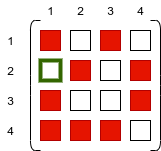
\includegraphics[width=0.45\textwidth]{./Scheduler/PpT-Symbolic_A01.png}
\end{minipage}%
\hfill
\begin{minipage}{0.85\textwidth}
According to equation \ref{eqn:LUD:LUequation1},\\
$L_{2,1}=0$
\end{minipage}

\begin{minipage}{0.45\textwidth}
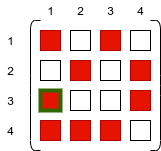
\includegraphics[width=0.45\textwidth]{./Scheduler/PpT-Symbolic_A02.png}
\end{minipage}%
\hfill
\begin{minipage}{0.85\textwidth}
According to equation \ref{eqn:LUD:LUequation1},\\
$L_{3,1}=A_{3,1}/U_{1,1}$
\end{minipage}

\begin{minipage}{0.45\textwidth}
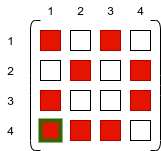
\includegraphics[width=0.45\textwidth]{./Scheduler/PpT-Symbolic_A03.png}
\end{minipage}%
\hfill
\begin{minipage}{0.85\textwidth}
According to equation \ref{eqn:LUD:LUequation1},\\
$L_{4,1}=A_{4,1}/U_{1,1}$
\end{minipage}
\\\\
\textbf{Column 2: -}

\begin{minipage}{0.45\textwidth}
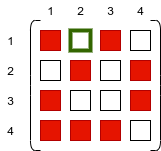
\includegraphics[width=0.45\textwidth]{./Scheduler/PpT-Symbolic_A10.png}
\end{minipage}%
\hfill
\begin{minipage}{0.85\textwidth}
According to equation \ref{eqn:LUD:LUequation0},\\
$U_{1,2}=0$
\end{minipage}

\begin{minipage}{0.45\textwidth}
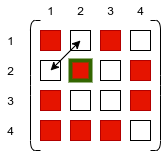
\includegraphics[width=0.45\textwidth]{./Scheduler/PpT-Symbolic_A11.png}
\end{minipage}%
\hfill
\begin{minipage}{0.85\textwidth}
According to equation \ref{eqn:LUD:LUequation0},\\
$U_{2,2}=A_{2,2}$
\end{minipage}

\begin{minipage}{0.45\textwidth}
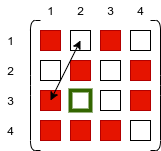
\includegraphics[width=0.45\textwidth]{./Scheduler/PpT-Symbolic_A12.png}
\end{minipage}%
\hfill
\begin{minipage}{0.85\textwidth}
According to equation \ref{eqn:LUD:LUequation1},\\
$L_{3,2}=0$
\end{minipage}

\begin{minipage}{0.45\textwidth}
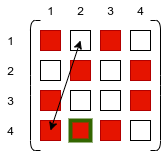
\includegraphics[width=0.45\textwidth]{./Scheduler/PpT-Symbolic_A13.png}
\end{minipage}%
\hfill
\begin{minipage}{0.85\textwidth}
According to equation \ref{eqn:LUD:LUequation1},\\
$L_{4,2}=A_{4,2}/U_{2,2}$
\end{minipage}
\\\\
\textbf{Column 3: -}

\begin{minipage}{0.45\textwidth}
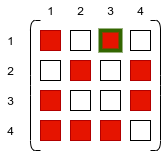
\includegraphics[width=0.45\textwidth]{./Scheduler/PpT-Symbolic_A20.png}
\end{minipage}%
\hfill
\begin{minipage}{0.85\textwidth}
According to equation \ref{eqn:LUD:LUequation0},\\
$U_{1,3}=A_{1,3}$
\end{minipage}

\begin{minipage}{0.45\textwidth}
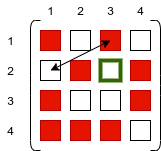
\includegraphics[width=0.45\textwidth]{./Scheduler/PpT-Symbolic_A21.png}
\end{minipage}%
\hfill
\begin{minipage}{0.85\textwidth}
According to equation \ref{eqn:LUD:LUequation0},\\
$U_{2,3}=0$
\end{minipage}


\begin{minipage}{0.45\textwidth}
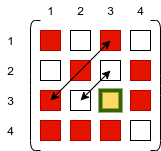
\includegraphics[width=0.45\textwidth]{./Scheduler/PpT-Symbolic_A22.png}
\end{minipage}%
\hfill
\begin{minipage}{0.85\textwidth}
According to equation \ref{eqn:LUD:LUequation0},\\
$U_{3,3}=-(L_{3,1} \cdot U_{1,2})$
\end{minipage}

\begin{minipage}{0.45\textwidth}
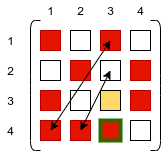
\includegraphics[width=0.45\textwidth]{./Scheduler/PpT-Symbolic_A23.png}
\end{minipage}%
\hfill
\begin{minipage}{0.85\textwidth}
According to equation \ref{eqn:LUD:LUequation1},\\
$ L_{4,3}=A_{4,3} - ( L_{4,1} \cdot U_{1.3} )/U_{3,3} $
\end{minipage}
\\\\
\textbf{Column 4: -}

\begin{minipage}{0.45\textwidth}
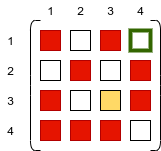
\includegraphics[width=0.45\textwidth]{./Scheduler/PpT-Symbolic_A30.png}
\end{minipage}%
\hfill
\begin{minipage}{0.85\textwidth}
According to equation \ref{eqn:LUD:LUequation0},\\
$U_{1,4}=0$
\end{minipage}

\begin{minipage}{0.45\textwidth}
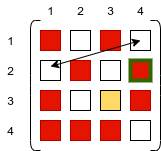
\includegraphics[width=0.45\textwidth]{./Scheduler/PpT-Symbolic_A31.png}
\end{minipage}%
\hfill
\begin{minipage}{0.85\textwidth}
According to equation \ref{eqn:LUD:LUequation0},\\
$U_{2,4}=A_{2,4}$
\end{minipage}

\begin{minipage}{0.45\textwidth}
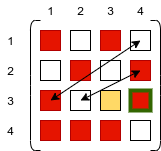
\includegraphics[width=0.45\textwidth]{./Scheduler/PpT-Symbolic_A32.png}
\end{minipage}%
\hfill
\begin{minipage}{0.85\textwidth}
According to equation \ref{eqn:LUD:LUequation0},\\
$U_{3,4}=A_{3,4}$
\end{minipage}

\begin{minipage}{0.45\textwidth}
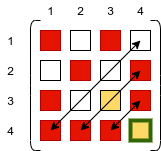
\includegraphics[width=0.45\textwidth]{./Scheduler/PpT-Symbolic_A33.png}
\end{minipage}%
\hfill
\begin{minipage}{0.85\textwidth}
According to equation \ref{eqn:LUD:LUequation0},\\
$U_{4,4}= - (L_{4,2}\cdot U_{2,4} + L_{4,3}\cdot U_{3,4})$
\end{minipage}
\\
\\
This would be resulting in the \ref{fig: Symbolic_complete} in terms of non-zero matrix locations. As we can see that there are new locations (colored yellow) while decomposing the matrix.

\begin{figure}[H]
    \centering
    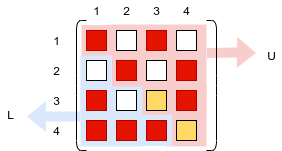
\includegraphics[width = 0.40\textwidth]{./Scheduler/PpT-Symbolic_Complete.png}
    \caption{Non-zero location of Matrix}
    \label{fig:Symbolic_complete}
\end{figure}

\section{Priority Ordering}

Proper priority assignment is beneficial for optimal schedule generation. For resolving contention, scheduling should be assigned the highest priority to the specific nodes. Priority assignment starts from root nodes, and we gradually move towards the leaf nodes. The memory read should be given more priority to the floating-point operations. The priority is defined as:
\begin{tcolorbox}
\begin{equation*}
    \centering
    Priority(n) = \sum_{i \in Parents(n)} Priority(i) + \sum_{x \in tasks(n)} Delay(x)
\end{equation*}
\end{tcolorbox}

where $Parents(n)$ is the set of node which are dependent on the node $n$ and $tasks(n)$ is the set of operations to evaluate the node $n$.This definition nodes will prioritized by the greedy scheduling  algorithm.

The priority calculation formula for node of type “/”(DIV) is given below: -
\begin{equation*}
    \centering
    ''/” node priority = \sum_{i \in Parents(n)} Priority(i) + latency_{DIV}
\end{equation*}

The priority calculation formula for node of type “mac\_sub”(MAC) is given below: -
\begin{equation*}
    \centering
    ''mac\_sub” node priority = \sum_{i \in Parents(n)} Priority(i) +\#MAC\_operations \times latency_{MAC}
\end{equation*}

Using The Priority ordering and Symbolic analysis in \ref{fig:Symbolic_1},  the Following DAG is generated, \ref{fig:DAG_gen}
\begin{figure}[H]
    \centering
    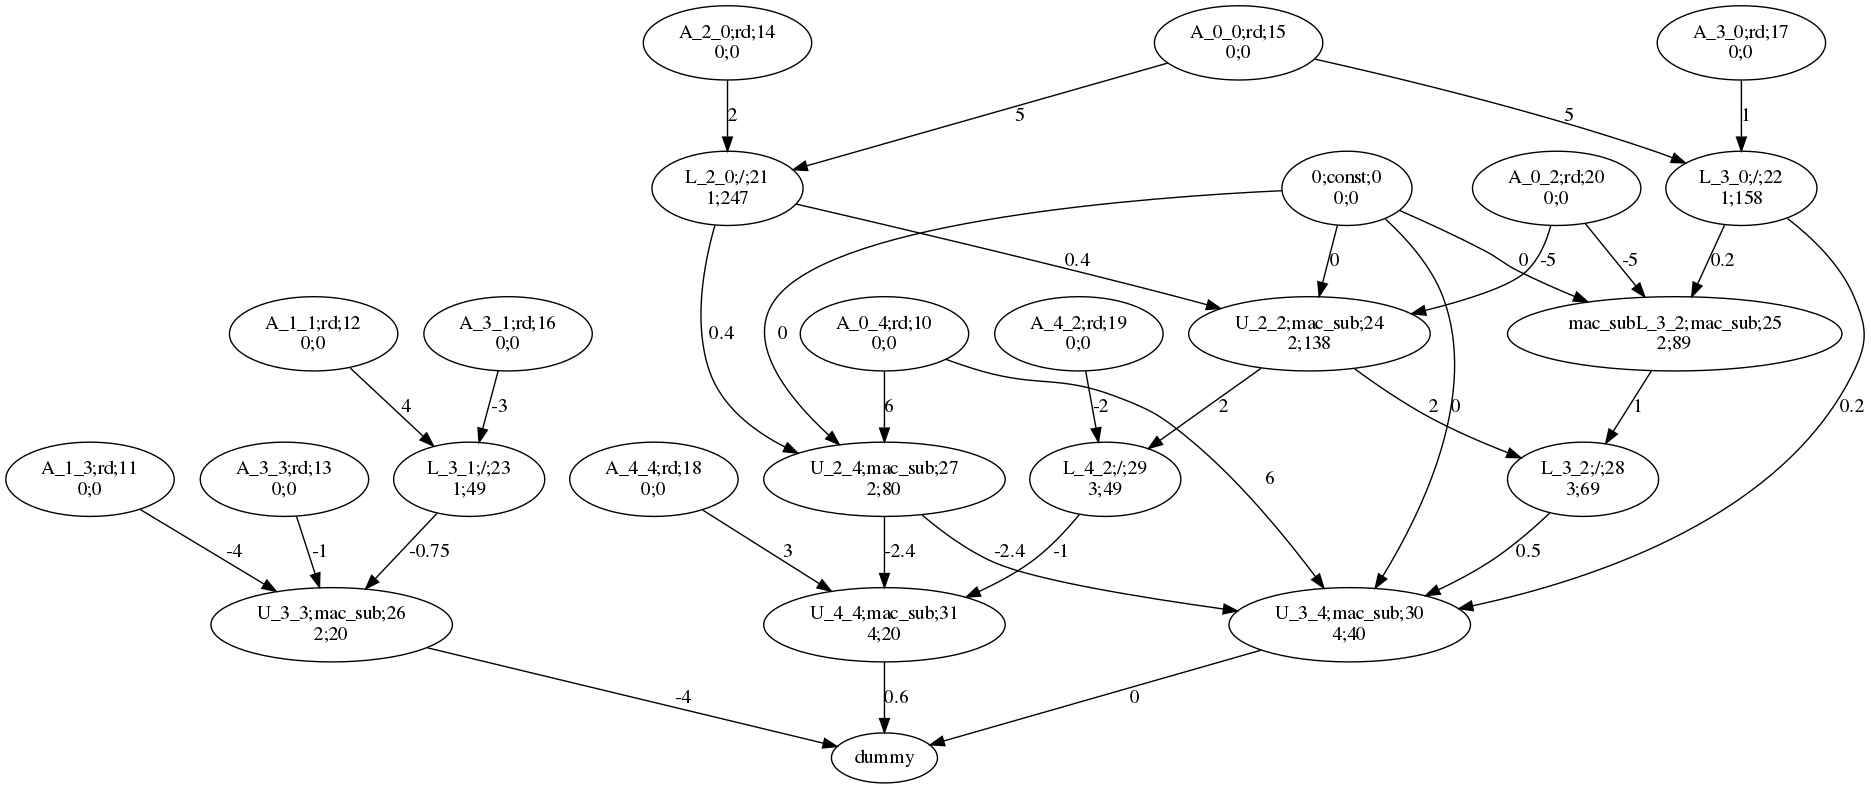
\includegraphics[width = 0.75\textwidth]{./Scheduler/exeTree.png}
    \caption{Generated DAC}
    \label{fig:DAG_gen}
\end{figure}

The meaning of terms inside each node of the data flow graph is described in the figure \ref{fig:DAG_mean} below: -
\begin{figure}[H]
    \centering
    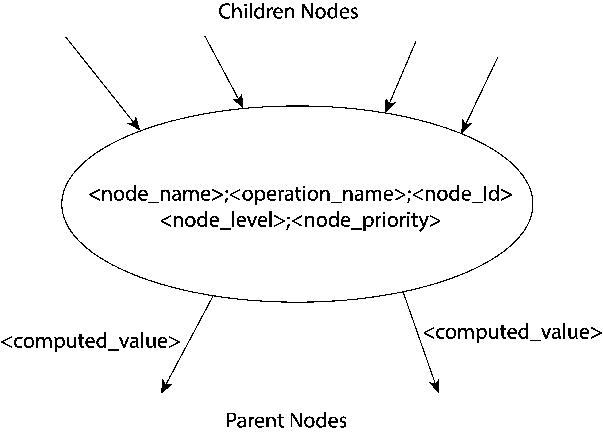
\includegraphics[width = 0.55\textwidth]{./Scheduler/image45.png}
    \caption{DAC node convention}
    \label{fig:DAG_mean}
\end{figure}
Note the convention used by children nodes and parent nodes in this project. Nodes which are providing a value to a given node are \textbf{children} of the given node. And the nodes which are accepting value from a given node are \textbf{parents} to the given node

\begin{description}
    \item[<node\_name>:] Indicates the name associated with the node. he node name is of the form ``L\_x\_y",``U\_x\_y", ``mac\_subL\_x\_y" etc. The ``node\_name" is unique.
    \item[<operation\_name>:] Indicates the operation performed by the node. The operations can be ``rd”(memory read), ``wr”(memory write), ``mac\_sub” (MAC), ``/”(DIV) or ``const” (indicates that the node has a constant value of 0).
    \item[<node\_Id>:] Indicates a unique Id associated with each node.
    \item[<node\_level>:] Indicates the level of the node i.e. the worst-case distance from a leaf node.
    \item[<node\_priority>:] It indicates the priority level of the node. This parameter is extremely useful while scheduling the graph.
    \item[<computed\_value>:] This parameter indicates the value computed by the node. Ex. $U_{1,1} = 5$, $U_{2,3} = -2.65$ etc.
\end{description}

\section{Priority List Based Scheduling}

The basic idea of list scheduling is to make an ordered list of processes by assigning them  priorities and then repeatedly execute the following steps until a valid schedule is obtained :
\begin{itemize}
        \item Select from the list the process with the highest priority for scheduling.
        \item Select a resource to accommodate this process.
        \item If no resource can be found, we select the following process in the list.
\end{itemize}
Considering an example.We have following which are pipeline in nature mentioned in \ref{fig:Example_graph} 2 DIV units(latency = 2) and 2 MUL units(latency = 1)
\begin{figure}[H]
    \centering
    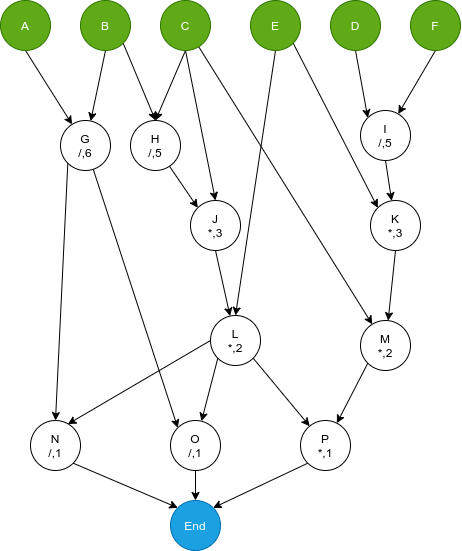
\includegraphics[width = 0.55\textwidth]{./Scheduler/PpT-Scheduler_Example_graph.png}
    \caption{Priority-Based Algorithm}
    \label{fig:Example_graph}
\end{figure}
For demonstrating list scheduling with this graph, I have considered four lists ''schedulable\_list,”
''execution\_list” \& ''cyclesLeft\_list”. The last two lists go hand in hand. The contents of these lists
in each cycle is given below: -\\
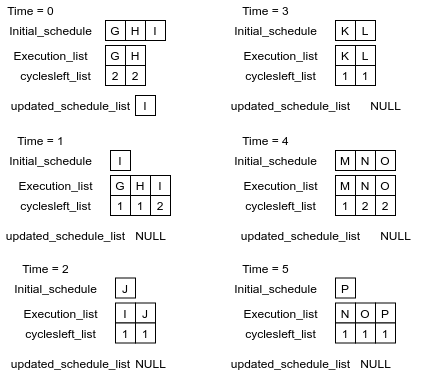
\includegraphics[width=0.85\textwidth]{./Scheduler/PpT-Scheduler_Example_graph_ALL.png}
\\
The concept behind list scheduling used in this project is same as the above example although included some of the real constraints
\begin{itemize}
    \item All the operand are fetch from memory i.e. limited number of ports
    \item Handling Live of operands
    \item Resource Binding of Processing elements
\end{itemize}
Therefore following are the inputs to the Scheduler
\begin{itemize}
    \item Number of BRAM blocks
    \item Number of ports per BRAM block
    \item Number of MAC and DIV units
    \item Latencies of MAC and DIV units
\end{itemize}

The important steps in the algorithm are as follows:

\begin{algorithm}[H]
    \caption{Priority List based Scheduling Process}
        \label{algo:sch:sch}
    \begin{algorithmic}[1]
        \Require{$G$, a computation flow graph for LU decomposition}
        \Statex
        \State $scheduledNodes := 0$
        \State $readyNodes := G.leaves()$
        \While{$scheduledNodes < G.size()$}
            \State Update status of nodes retired in previous cycle
            \State Update scheduledNodes
            \State Update the ready nodes list
            \State Assign memory port to retiring nodes
            \State Calculate the free BRAM ports for reading and writing
            \State Select the most prior set of ready nodes which can be schedules in current cycle
            \State Assign the memory memory operations
        \EndWhile
    \end{algorithmic}
\end{algorithm}
The above Concept can be explainable by following flow chart figure \ref{fig:sch:Flowchart}
\begin{figure}[H]
    \centering
    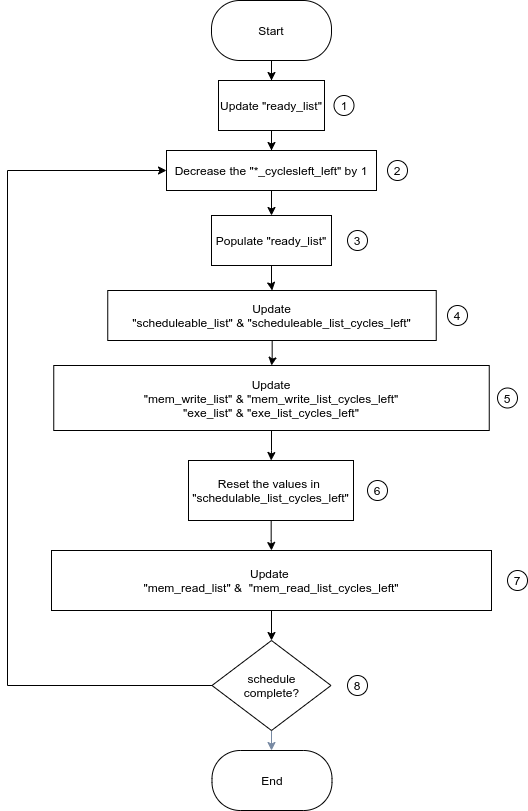
\includegraphics[width = 0.5 \textwidth]{./Scheduler/Flowchart.png}
    \caption{Flowchart of Priority List based Scheduling Process \cite{AnuragWork}}
    \label{fig:sch:Flowchart}
\end{figure}

The scheduling algorithm uses three tables, namely the assignment table, retirement table, and memory operation table, to track all assigned operations and determine the next set of assignments. The scheduler cycle-accurate simulation and stores the assignment as a set of instructions for hardware.\cite{AnuragWork}
\begin{figure}[H]
    \centering
    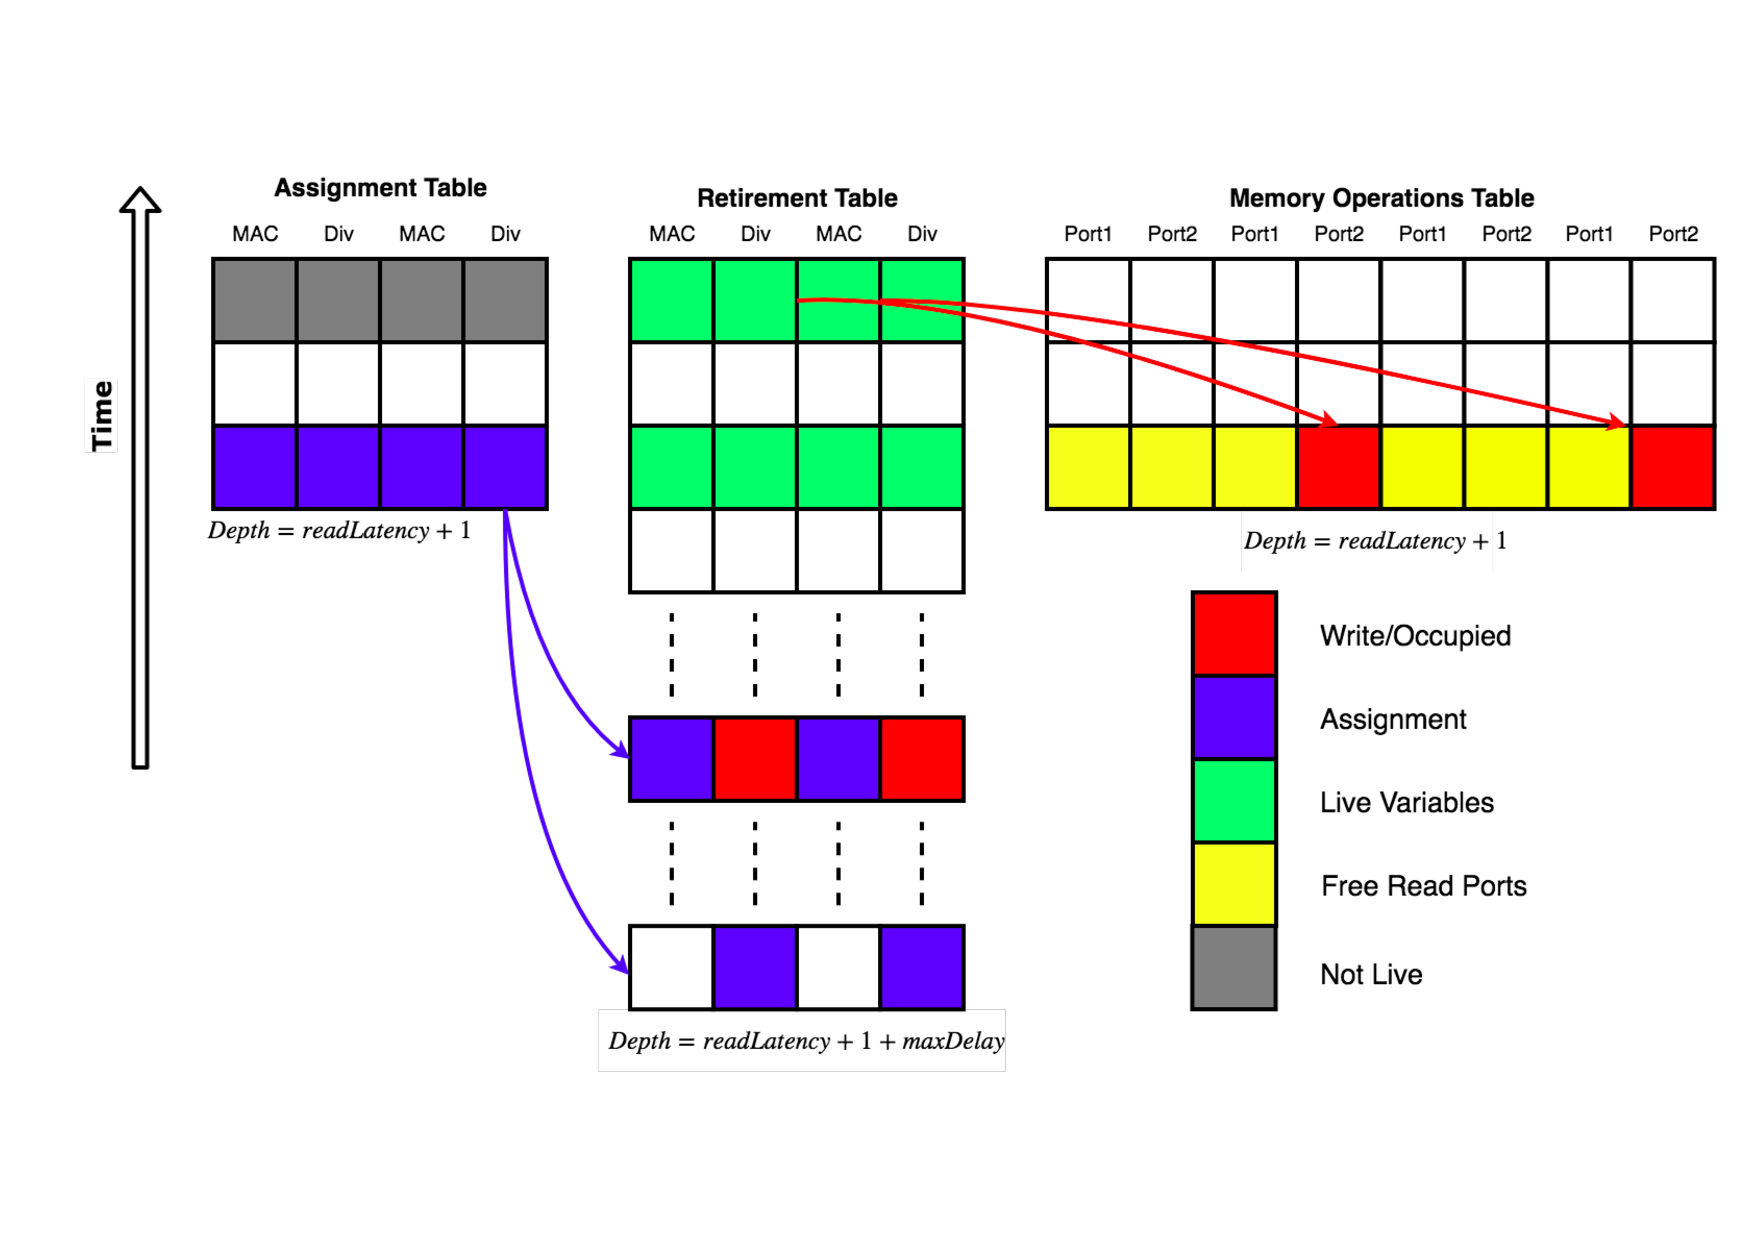
\includegraphics[width = \linewidth]{./Scheduler/schedulartable.pdf}
    \caption{Allocation tables used by scheduling algorithm \cite{YogeshWork}}
    \label{fig:sch:tableBlank}
\end{figure}

\textbf{Assignment Table:}\\
All the operations scheduled in a cycle must store in the same cycle they return because of the unavailability of the output buffer—the corresponding retirement table used for removing duplication of entries in the cell. The size of the Assignment Table is equal to the number of MAC \& DIV units with reading latency. The read latency can be two as it will be virtual if Quad-port Data BRAM is used; else, it would be one.
\\
\\
\textbf{Retirement Table:}\\
The operations are retiring in the current cycle, i.e., operations whose results are available on the output ports of PEs. These results must
be written to the memory except in the case of write cancellation.
\\
\\
\textbf{Memory Operation Table:}\\
Memory Operation Table serves to maintain a record of available ports and assigned operations. Operation is assigned to particular Data BRAM from the time-multiplexed ports.
\\
\\
\textbf{Selecting the set of assignments:}
All the schedulable nodes are stored in a priority list in decreasing order. All combinations of nodes are checked availability of BRAM ports for both reading and retirement. A valid combination with the highest sum of priorities is selected as an assignment for the current cycle.
\\
\\
The required number of readings and writes corresponding to each node for each Data RAM will be listed in the adjoining tables. A good group of operations must have the sum of ports required, but the selected node should be less than the total available nodes. The set with a maximum sum of priority would be assigned to Processing elements in the current cycle.The additional required data values are set to be read from corresponding memory locations read allocation table.
\\
\\
The Scheduling process will be recursively working till the dummy node of the sequential graph is not reached. The final allocations of resources and processes are recorded for every timestamp, and instructions are generated. These instructions are in the form of bits that will be pass through instruction BRAM to the crossbar switch for executions.

